\documentclass[a4paper]{article}

\usepackage[english]{babel}
\usepackage[utf8x]{inputenc}
\usepackage{amsmath}
\usepackage{graphicx}
\usepackage[colorinlistoftodos]{todonotes}

\title{Project Report \\ News System  \\ EDA031 C++ Programming}
\date{\today}
\author{Christian Andersen \\ dat11can@student.lu.se \and Ragnar Mellbin \\ dat11rme@student.lu.se \and Fredrik Paulsson \\ dat11fp1@student.lu.se
\and Felix \AA kerlund \\ dat11fak@student.lu.se}
%\setcounter{secnumdepth}{5}
%\setcounter{tocdepth}{5}
\begin{document}
\clearpage\maketitle
\thispagestyle{empty}
\newpage

%\begin{abstract}
%Your abstract.
%\end{abstract}

\section{Introduction}
In this project we are to develop a client/server news system. There will be two version of the server, one version that saves it's data in the primary memory and one version that saves the data on the disk memory instead. The client will be simple with only a text based interface.

The server will store a list of newsgrous each identified with a unique ID. For each newsgroup the server will store a list of articles. The articles will be identified with each own ID that is unique for the newsgroup to which the article belongs.

This report serves as documentation of our project.

\section{Description of system design}

\includegraphics[width=\textwidth]{uml_seq}

Both the client and the server utilize the supplied \texttt{clientserver} library, and they are inspired by the supplied test programs.

\textbf{Enligt projektbeskrivningen: "A detailed description of your system design, both for the server and the clients. Preferably
use UML diagrams to give an overview of the design. (It is not necessary that you list
attributes and methods in these diagrams.) You must also describe the classes, at least as
far as stating the responsibilities of each class. Also give an overview of the dynamics of the server, i.e., trace an interaction between a
client and the server from the point that the server receives a command until it sends the
reply. UML sequence diagrams are good for this purpose."}

\subsection{Server}

The server consists of five parts. Entities representing newsgroups and articles, a database keeping track of these, a server which handles connections and a message handler which does the communication with the client.

The only difference between the two sever programs is the type of the database attribute, they are identical in all other regards.

\subsubsection{In-Memory Server}

This version of the server uses the class called \texttt{MemoryDatabase} to store information about all newsgroups and articles.

The unique thing about this database is that it stores all data in memory and thus looses all data upon shutdown. In order to store the data in memory it keeps four data structures to organize the data. It has a counter for the newgroup ID:s and a map mapping newsgroup ID:s to counters for article ID:s within each newsgroup. These counters are never decreased when objects are removed and increased whenever objects are added. This is what ensures that ID:s are unique for each object created.

The newsgroups are stored in a map, mapping ID to newsgroup. Articles are stored in a map within a map, mapping from newsgroup ID to a map mapping article ID:s to articles.

In these data structures two simple classes are stored, namely, \texttt{Newsgroup} and \texttt{Article}. ID:s are stored as integers in the form of \texttt{size\_t}.


\subsubsection{On-Disk Server}
The diskserver stores information on the disk \emph{only}. Every time data is requested it is read from the disk, and every read is written to the disk. While this is significantly slower than keeping the database in the memory alongside the disk, we do not risk running out of memory as the database grows.

The information is stored in a specific folder, where each group has its own folder, and each article has its own folder inside these. There are also files used for keeping track of the groupnames in use, as well as for keeping track of the last inserted group and article ID:s.

\subsection{Client}
The client is divided into four parts. These four parts consists of two classes, one struct and a file containing a few methods including the \texttt{main}-method of the client itself. Two of these parts were provided. An overview of the client parts is shown in figure \ref{clientUML}.

\begin{figure}
    \centering
    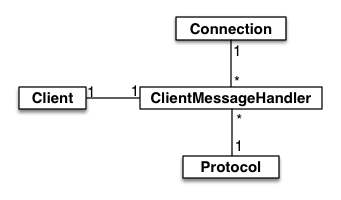
\includegraphics[width=0.6\textwidth]{projectUML-client.png}
    \caption{UML diagram client the client}
    \label{clientUML}
\end{figure}

We have developed the two parts named \texttt{Client} and \texttt{ClientMessageHandler}. The parts named \texttt{Connection} and \texttt{Protocol} were given to us when we started the development.

The \texttt{Connection} class simply describes a connection to the server part and has methods which allows us to write messages to the server. The \texttt{Protocol} struct defines constants used in the protocol that were specified for us.

The \texttt{ClientMessageHandler} uses a \texttt{Connection} and the constants defined in \texttt{Protocol} in order to send commands to the server and present the responses. Every action that the client can issue to the server is represented as a single method in the \texttt{ClientMessageHandler} class. For instance, it has methods such as \texttt{createNewsgroup}, \texttt{deleteNewsgroup}, \texttt{createArticle} and \texttt{getArticle} among others. This class also contains some private helper methods used to read and write strings and numbers received from and sent to the server.

The file named \texttt{Client} contains the \texttt{main}-method of the client and handles interaction with the user. For example, this file contains methods such as \texttt{queryUserMenu}, \texttt{promptInt}, \texttt{promptString} and \texttt{interact}. These methods are fairly straightforward, the prompt methods are simply helper functions used to request input from the user. \texttt{queryUserMenu} displays a menu of all avialable actions to the user and asks for a selection. \texttt{interact} connects all functions together. It contains a loop that displays the menu and, depending on the selection, uses the prompt functions to gather input and finally calls the appropriate method in the \texttt{ClientMessageHandler} class. The \texttt{main}-method simply initializes the \texttt{ClientMessagehandler} and calls the \texttt{interact} function.

\section{Conclusions}
We fulfil all of the requirements listed in section 2 of the project description.


\textbf{Enligt projektbeskrivning:
"Requirements that you fulfill, problems that you haven’t succeeded in solving,
etc. If you have found that the system ought to have more features you should elaborate on
this. Any suggestions for improvements to the project are also welcome"}
\end{document}
